\section{Setup}
Before beginning, players must decide how many points to play to. 
We recommend 120 points for 2 players and 240 points for 3-4 players, but the actual number is ultimately up to you.
\subsection{2 Players}

\begin{enumerate}
    \item Flip all the dominoes face-down onto the table and give them a good shuffle.
    \item Arrange all the dominoes in 5 columns of 11
    \item Flip over the middle domino in each column.
\end{enumerate}

\subsection{3--4 Players}

\begin{enumerate}
    \item Flip all the dominoes face-down onto the table and give them a good shuffle.
    \item Arrange all the dominoes in 7 columns of 13
    \item Flip over the middle domino in each column.
\end{enumerate}

\begin{figure}[ht]
\centering
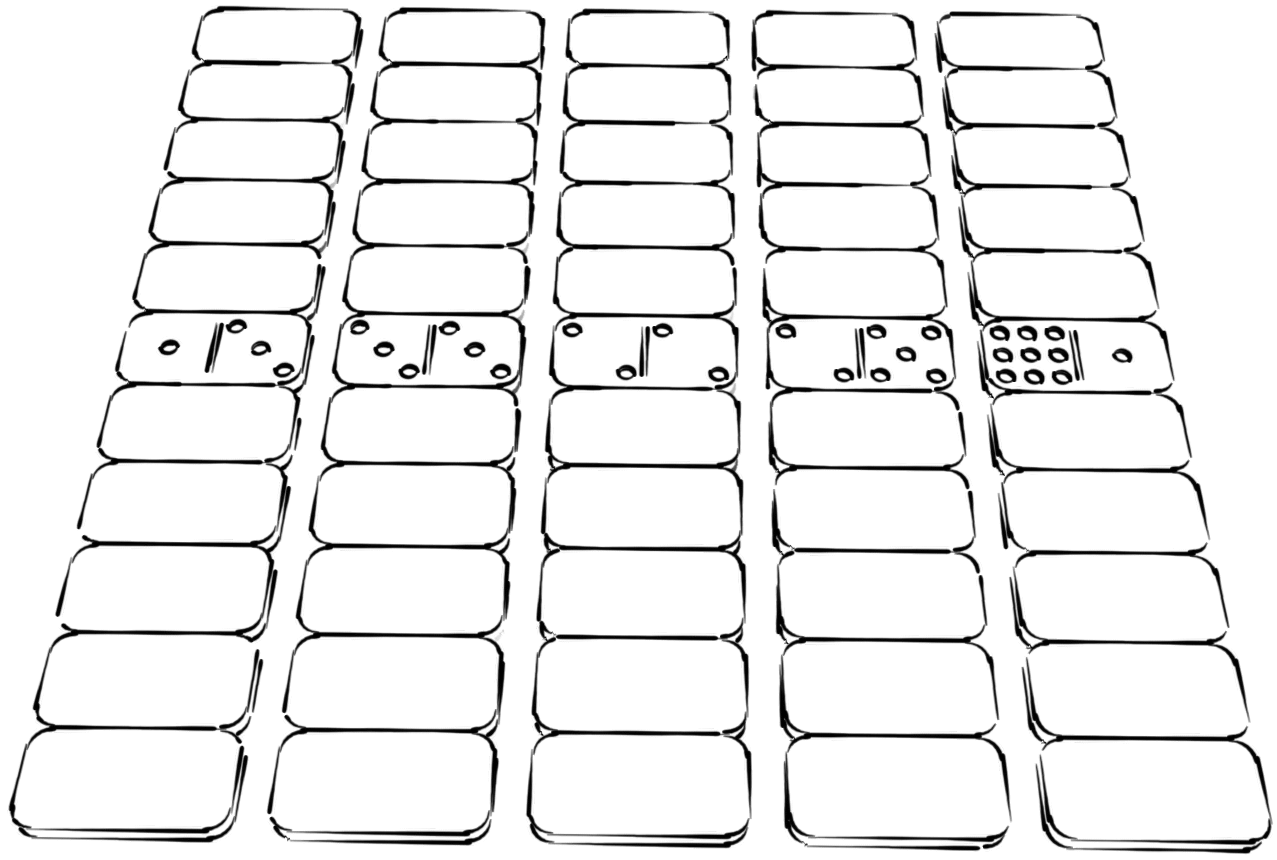
\includegraphics[width = \linewidth]{dominoes-setup.png}
\caption{Example setup for 2 players. 5 columns of 11 tiles.}
\end{figure}
\subsection{Selection Round}

Proceeding clockwise around the table, starting with the youngest player, a player may choose to either 
\begin{itemize} 
\item reveal one piece in any column
\item claim a column by taking all the pieces for themselves
\end{itemize}
Play starts once all players have each claimed one column.

\paragraph{Aside} The purpose of revealing pieces is to give players insight in what your starting hand may contain to perhaps give an advantage, and also to reveal some pieces you might be looking for later on. It also plays a little like a game of chicken---how many tiles do you dare reveal before someone else snatches the column you want?